\documentclass{article}
\usepackage{eecstex}
\usepackage{pgfplots}

\title{EE 123 HW 04}
\author{Bryan Ngo}
\date{2022-02-11}

\begin{document}

\maketitle

\setcounter{section}{2}

\section{}

\subsection{}

Each circular convolution in the overlap-save method will result in a length \(2^v - P + 1\) signal.
Then, the cost of the FFT and IFFT is \(\frac{2^v}{2} \log_2(2^v) = v 2^{v - 1}\).
Then, there is a \(2^v\)-pointwise multiplication.
The total number of multiplications is \(2^v (v + 1)\).
Thus, the FFT for each sample will require
\begin{equation}
    \frac{2^v (v + 1)}{2^v - P + 1}.
\end{equation}
complex multiplications per output sample.

\subsection{}

\begin{center}
    \begin{tikzpicture}
        \begin{axis}[
            xlabel=\(v\), ylabel={Cost},
            title={Complex Multiplications},
            axis lines=middle,
            width=0.4\textwidth
        ]
        \addplot[ycomb, mark=*, color=blue] table[
            col sep=comma,
            x=v, y=cost
        ]{q3.csv};
        \end{axis}
    \end{tikzpicture}
\end{center}
with a minimum cost of \(v = 12\).
The direct evaluation would cost \(500\) complex multiplications per output sample, since that is the length of a given sample.

\subsection{}

\begin{equation}
    \lim_{v \to \infty} \frac{2^v (v + 1)}{2^v - P + 1} = \lim_{v \to \infty} \frac{v + 1}{1 - \left(\frac{P - 1}{2^v}\right)} = v
\end{equation}
Thus, for \(P = 500\), the direct method will be more efficient for \(v > 500\).

\newpage
\section{Fun with FFT}

\begin{enumerate}
    \item For \(0 \leqslant k < N\), \(H[k] = X_r[k] + W_{2N}^k X_i[k]\).
    \item For \(0 \leqslant k < N\), \(H[k + N] = X_r[k] - W_{2N}^k X_i[k]\).
    \item \(X[k] = \frac{1}{2} (H[k] + H[k + N]) + \frac{j}{2} W_{2N}^{-k} (H[k] - H[k + N])\), which takes 3 multiplications and 3 additions.
\end{enumerate}

\newpage
\section{Hadamard Transform}

\subsection{}

\begin{equation}
    H_3 =
    \begin{bmatrix}
        1 & 1 & 1 & 1 & 1 & 1 & 1 & 1 \\
        1 & -1 & 1 & -1 & 1 & -1 & 1 & -1 \\
        1 & 1 & -1 & -1 & 1 & 1 & -1 & -1 \\
        1 & -1 & -1 & 1 & 1 & -1 & -1 & 1 \\
        1 & 1 & 1 & 1 & -1 & -1 & -1 & -1 \\
        1 & -1 & 1 & -1 & -1 & 1 & -1 & 1 \\
        1 & 1 & -1 & -1 & -1 & -1 & 1 & 1 \\
        1 & -1 & -1 & 1 & -1 & 1 & 1 & -1
    \end{bmatrix}
\end{equation}
The order that represents increasing frequency content is the sequency ordering.

\subsection{}

\newpage
\section{}

\subsection{}

\begin{align}
    X[3k] &= \sum_{n = 0}^{N - 1} x[n] W_N^{3kn} \\
    &= \sum_{n = 0}^{\frac{N}{3} - 1} x[n] W_N^{3kn} + \sum_{n = \frac{N}{3}}^{\frac{2N}{3} - 1} x[n] W_N^{3kn} + \sum_{n = \frac{2N}{3}}^{N - 1} x[n] W_N^{3kn} \\
    &= \sum_{n = 0}^{\frac{N}{3} - 1} x[n] W_N^{3kn} + \sum_{n = 0}^{\frac{N}{3} - 1} x\left[n + \frac{N}{3}\right] W_N^{3kn} + \sum_{n = 0}^{\frac{N}{3} - 1} x\left[n + \frac{2N}{3}\right] W_N^{3kn} \\
    &= \sum_{n = 0}^{\frac{N}{3} - 1} \left(x[n] + x\left[n + \frac{N}{3}\right] + x\left[n + \frac{2N}{3}\right]\right) W_N^{3kn} \\
    &= \sum_{n = 0}^{\frac{N}{3} - 1} \underbrace{\left(x[n] + x\left[n + \frac{N}{3}\right] + x\left[n + \frac{2N}{3}\right]\right)}_{x_1[n]} W_{\frac{N}{3}}^{kn}
\end{align}

\subsection{}

\begin{align}
    X[3k + 1] &= \sum_{n = 0}^{N - 1} x[n] W_N^{n(3k + 1)} \\
    &= \sum_{n = 0}^{\frac{N}{3} - 1} x[n] W_N^{n(3k + 1)} + \sum_{n = \frac{N}{3}}^{\frac{2N}{3} - 1} x[n] W_N^{n(3k + 1)} + \sum_{n = \frac{2N}{3}}^{N - 1} x[n] W_N^{n(3k + 1)} \\
    &= \sum_{n = 0}^{\frac{N}{3} - 1} x[n] W_N^{n(3k + 1)} + \sum_{n = 0}^{\frac{N}{3} - 1} x\left[n + \frac{N}{3}\right] W_N^{\frac{N}{3}} W_N^{n(3k + 1)} + \sum_{n = 0}^{\frac{N}{3} - 1} x\left[n + \frac{2N}{3}\right] W_N^{\frac{2N}{3}} W_N^{n(3k + 1)} \\
    &= \sum_{n = 0}^{\frac{N}{3} - 1} \left(x[n] + x\left[n + \frac{N}{3}\right] W_N^{\frac{N}{3}} + x\left[n + \frac{2N}{3}\right] W_N^{\frac{2N}{3}}\right) W_N^{n(3k + 1)} \\
    &= \sum_{n = 0}^{\frac{N}{3} - 1} \underbrace{\left(x[n] + x\left[n + \frac{N}{3}\right] W_N^{\frac{N}{3}} + x\left[n + \frac{2N}{3}\right] W_N^{\frac{2N}{3}}\right) W_N^n}_{x_2[n]} W_{\frac{N}{3}}^{kn} \\
    X[3k + 2] &= \sum_{n = 0}^{N - 1} x[n] W_N^{n(3k + 2)} \\
    &= \sum_{n = 0}^{\frac{N}{3} - 1} x[n] W_N^{n(3k + 2)} + \sum_{n = \frac{N}{3}}^{\frac{2N}{3} - 1} x[n] W_N^{n(3k + 2)} + \sum_{n = \frac{2N}{3}}^{N - 1} x[n] W_N^{n(3k + 2)} \\
    &= \sum_{n = 0}^{\frac{N}{3} - 1} x[n] W_N^{n(3k + 2)} + \sum_{n = 0}^{\frac{N}{3} - 1} x\left[n + \frac{N}{3}\right] W_N^{\frac{2N}{3}} W_N^{n(3k + 2)} + \sum_{n = 0}^{\frac{N}{3} - 1} x\left[n + \frac{2N}{3}\right] W_N^{\frac{4N}{3}} W_N^{n(3k + 2)} \\
    &= \sum_{n = 0}^{\frac{N}{3} - 1} \left(x[n] + x\left[n + \frac{N}{3}\right] W_N^{\frac{2N}{3}} + x\left[n + \frac{2N}{3}\right] W_N^{\frac{4N}{3}}\right) W_N^{n(3k + 2)} \\
    &= \sum_{n = 0}^{\frac{N}{3} - 1} \underbrace{\left(x[n] + x\left[n + \frac{N}{3}\right] W_N^{\frac{N}{3}} + x\left[n + \frac{2N}{3}\right] W_N^{\frac{2N}{3}}\right) W_N^{2n}}_{x_3[n]} W_{\frac{N}{3}}^{kn}
\end{align}

\subsection{}

\begin{center}
    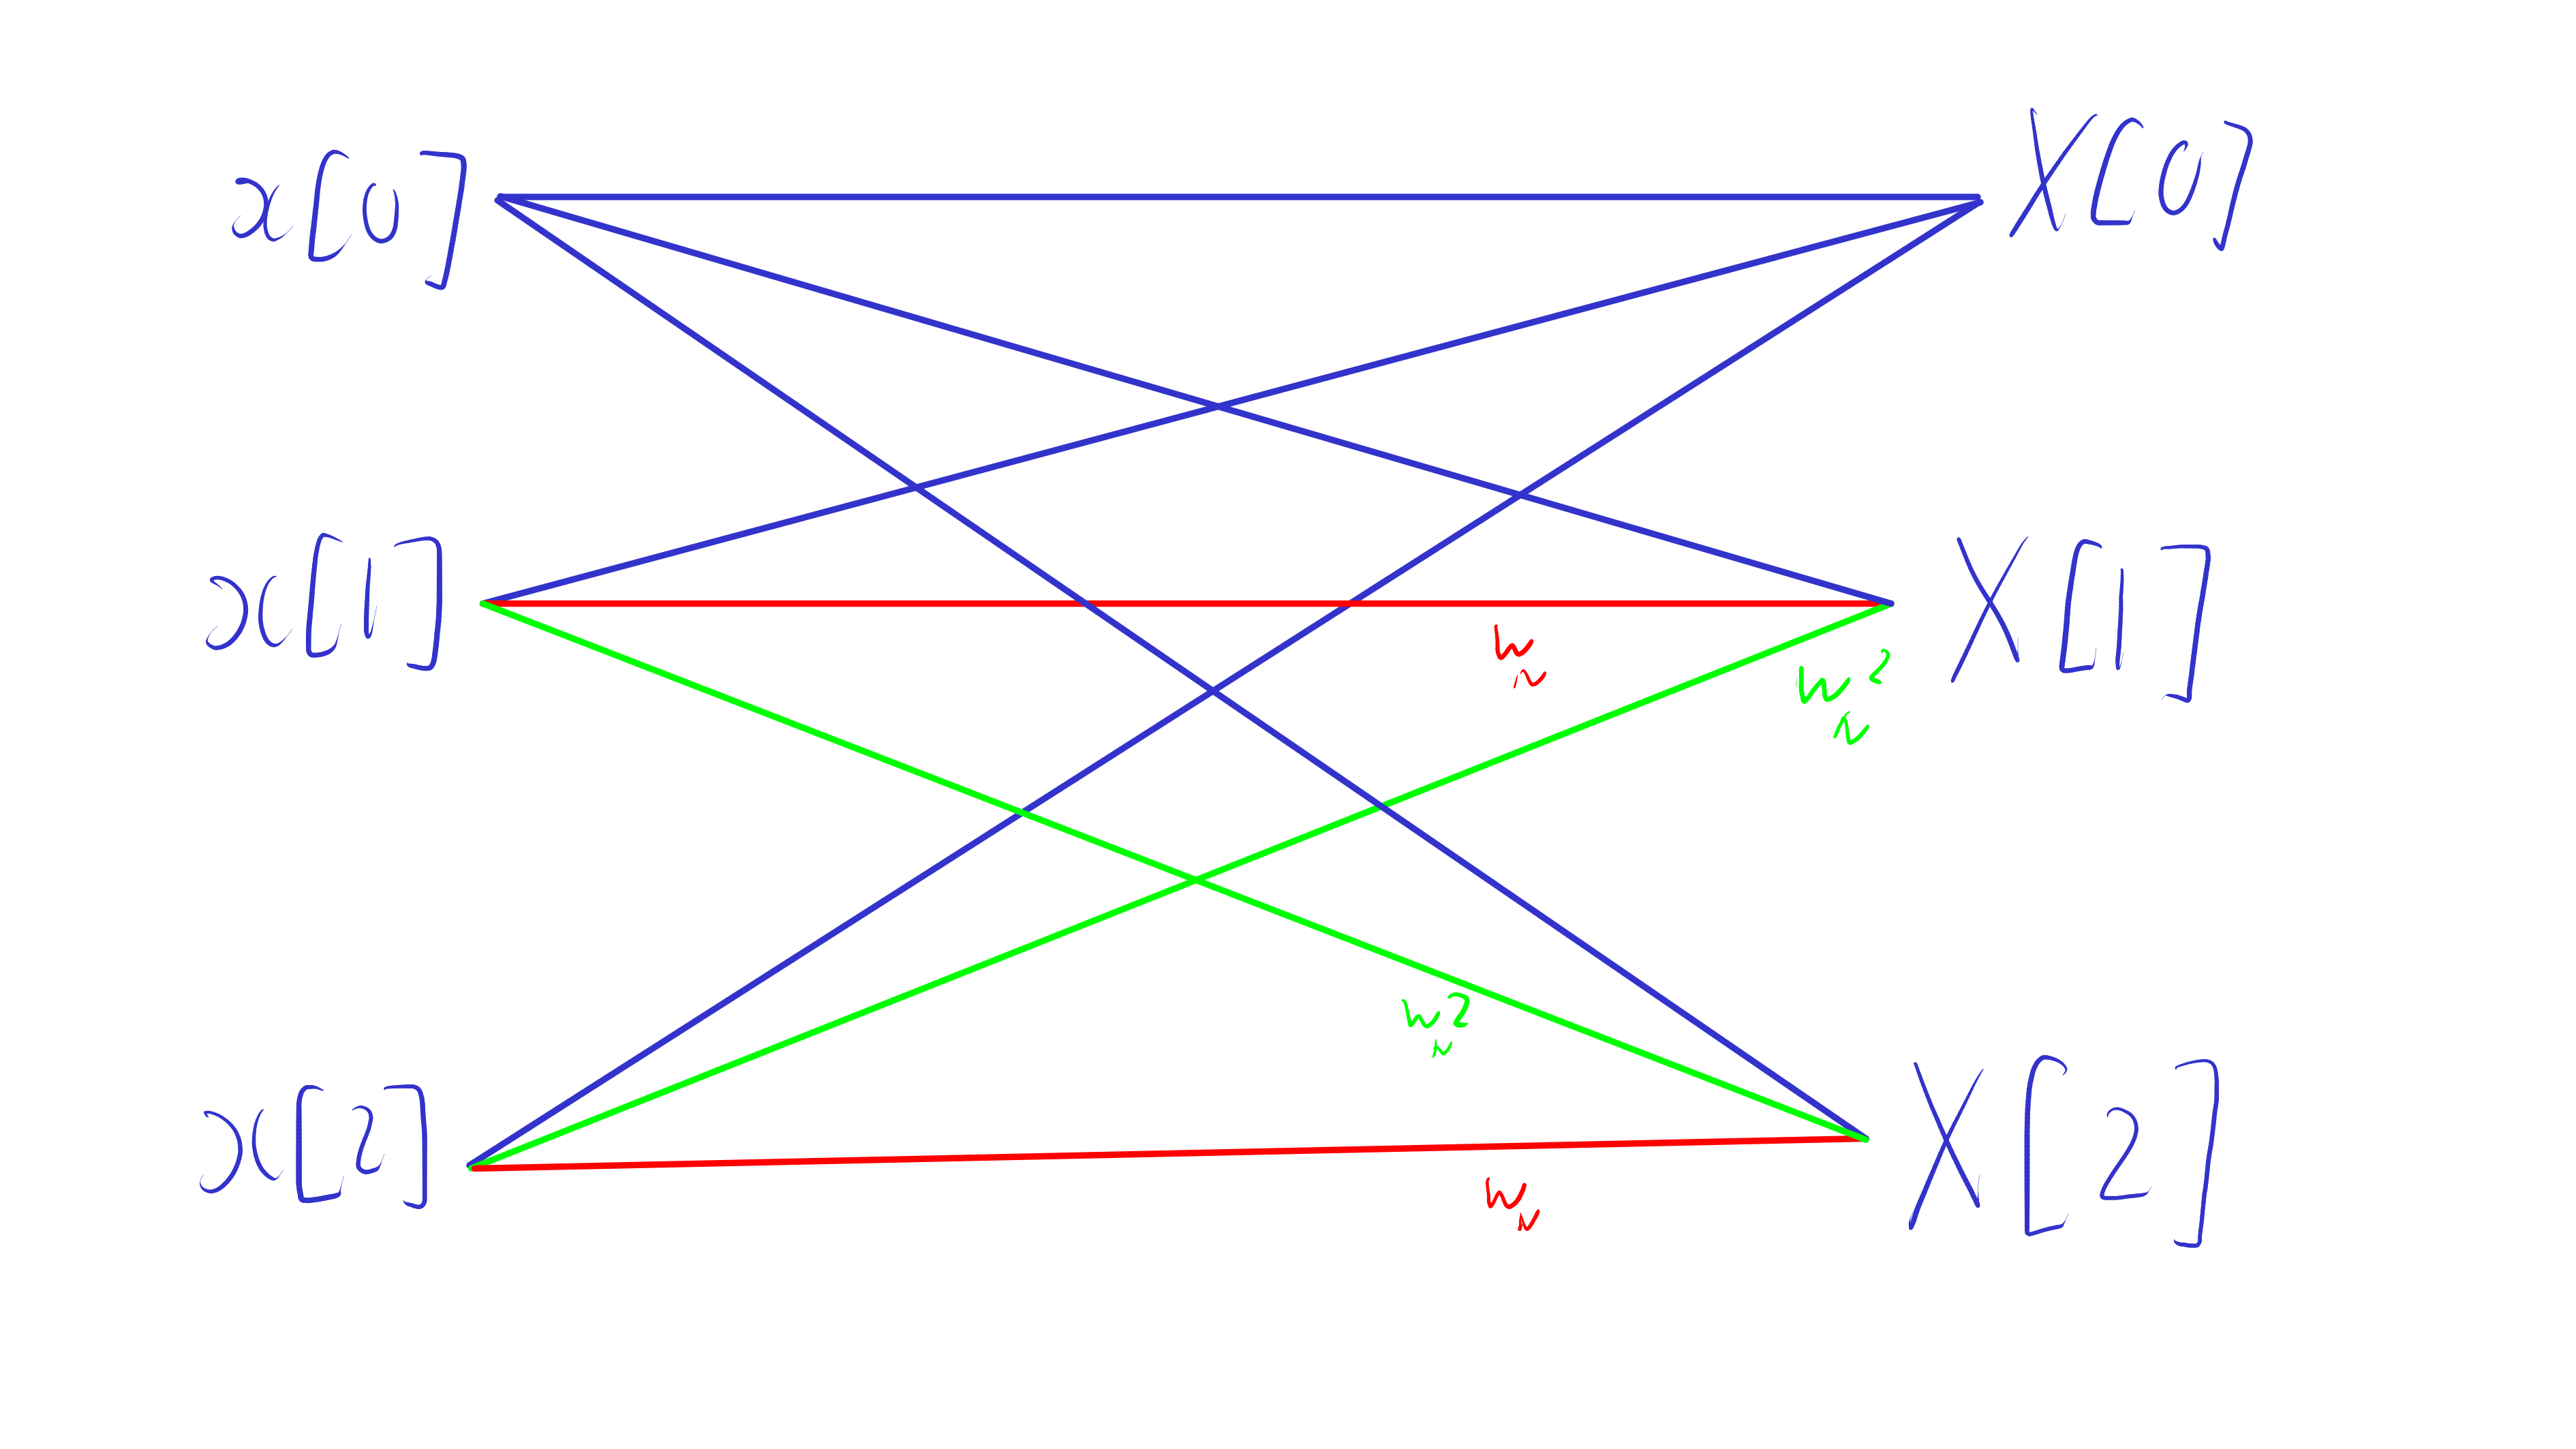
\includegraphics[width=0.7\textwidth]{q6c.png}
\end{center}

\subsection{}

\begin{center}
    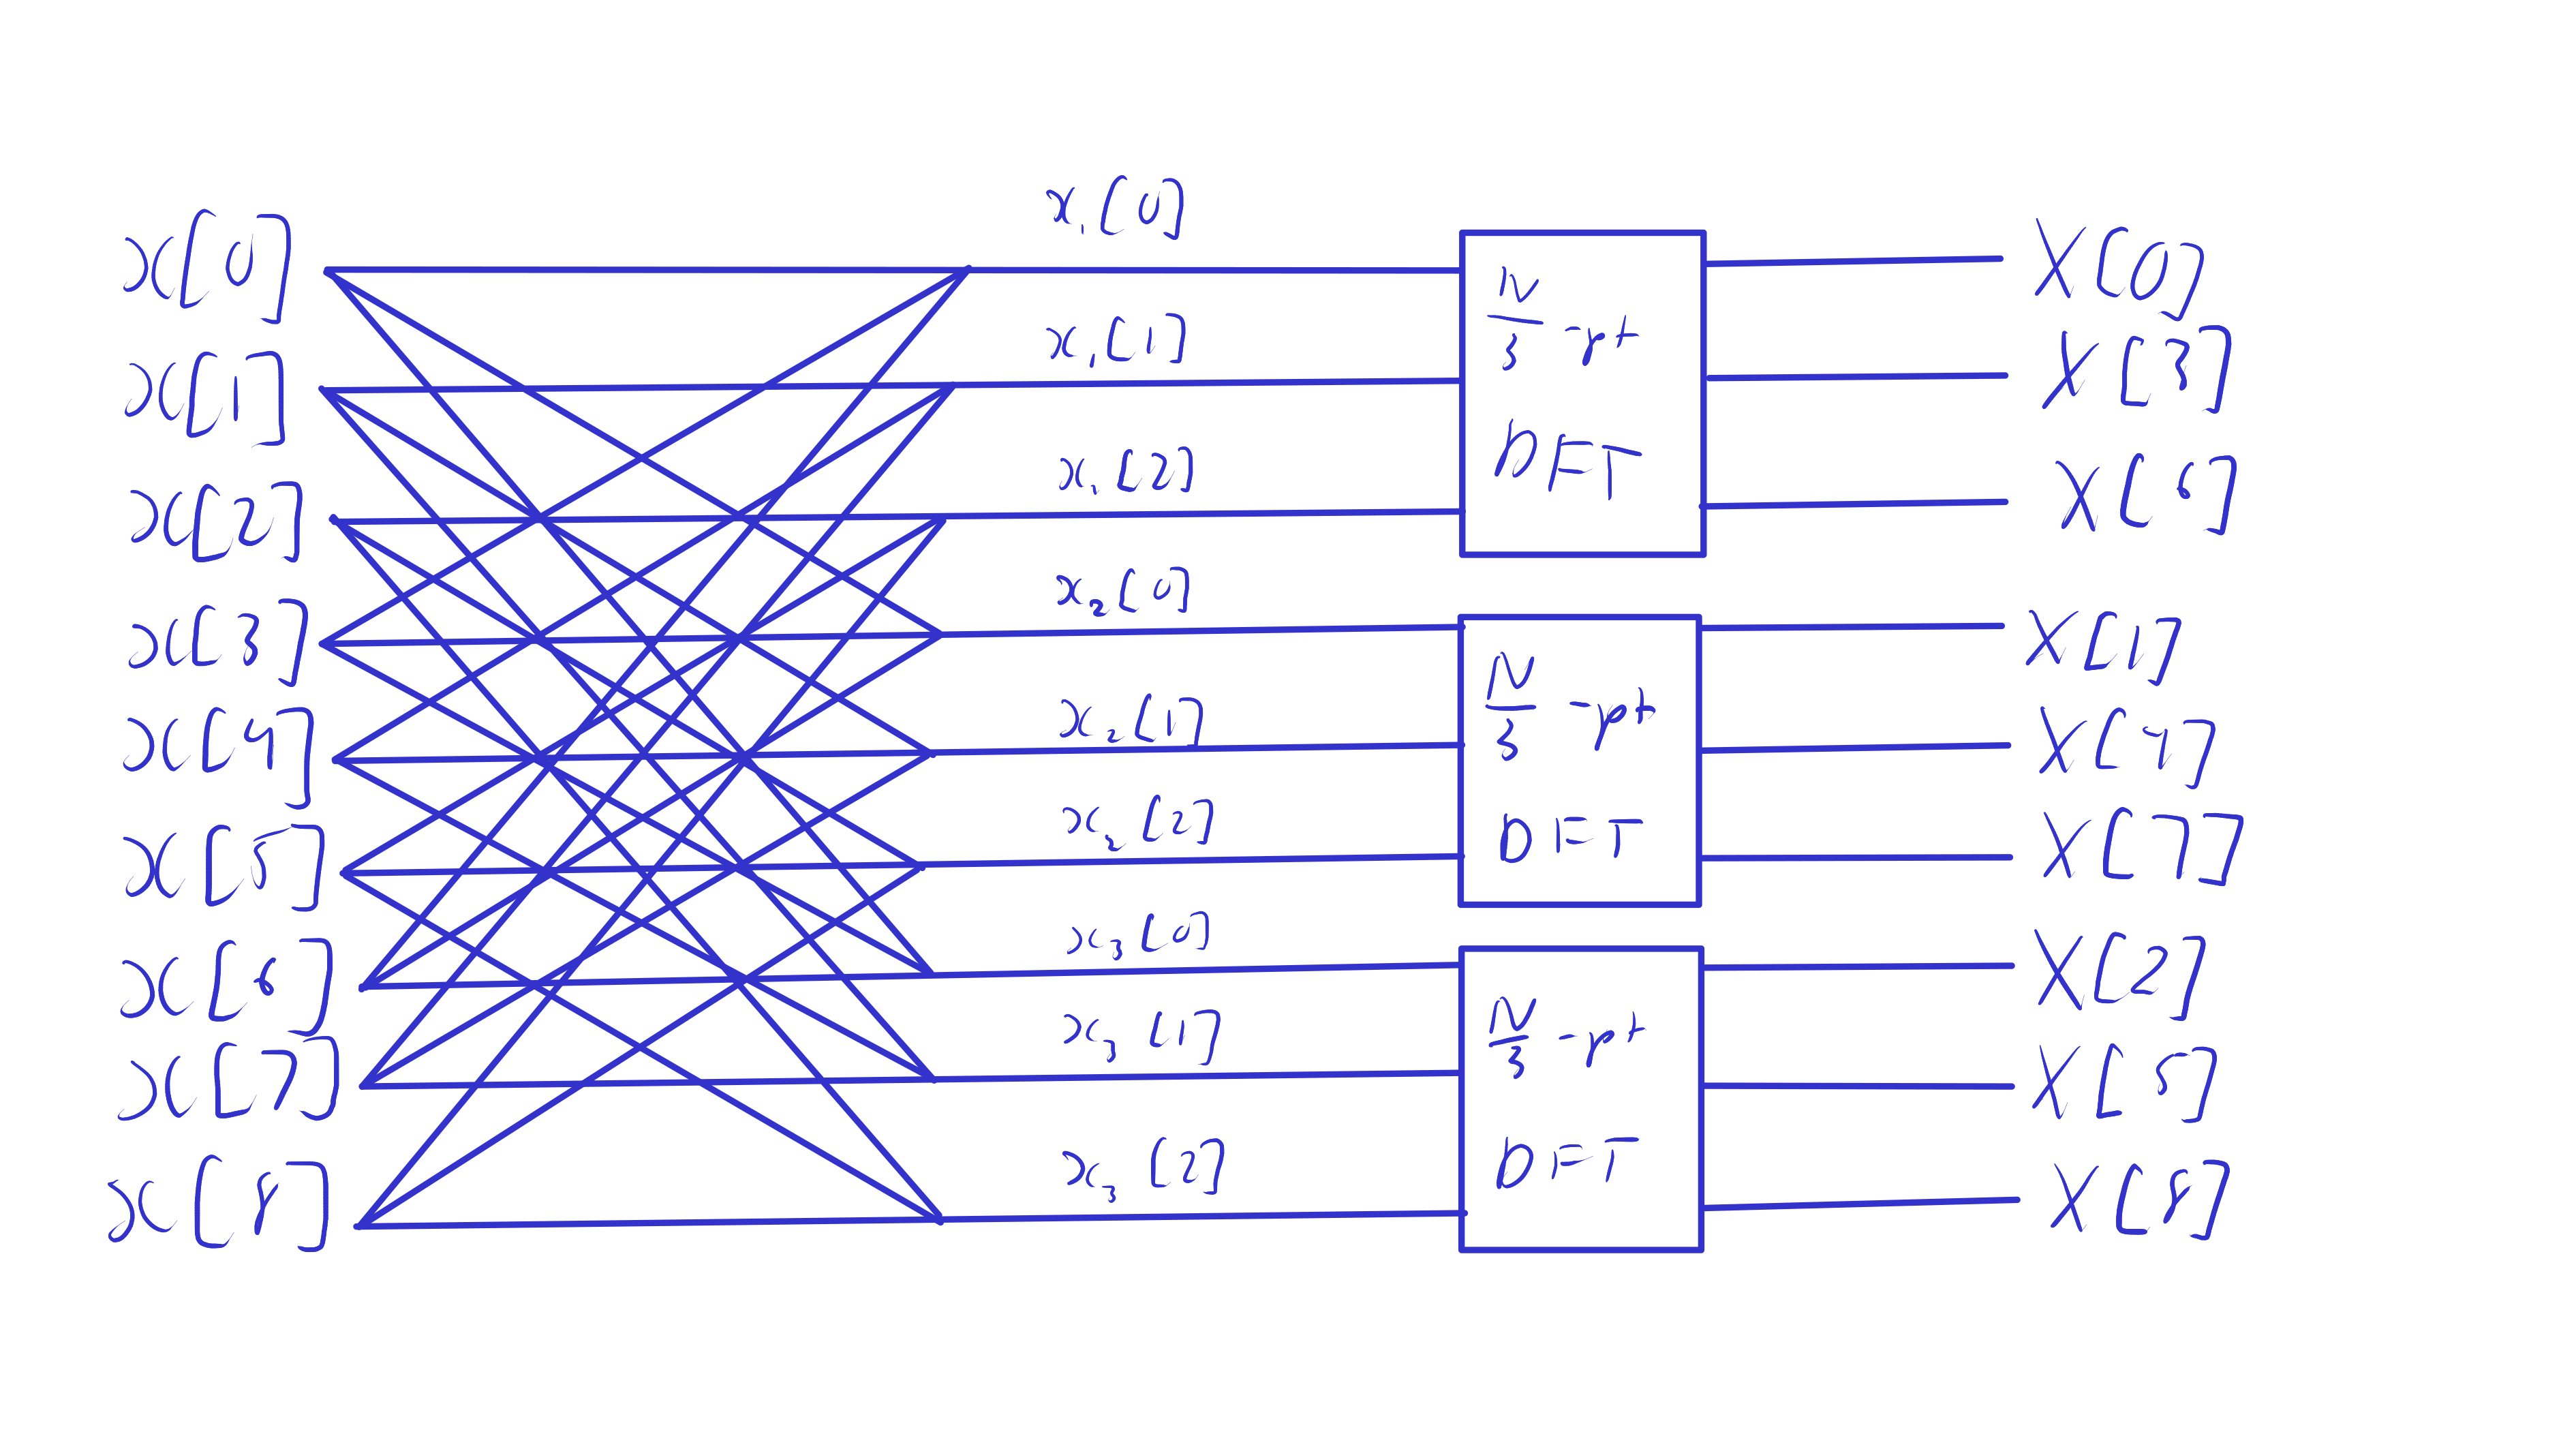
\includegraphics[width=0.8\textwidth]{q6d.png}
\end{center}

\newpage
\section{}

\begin{enumerate}
    \item \(|X[k]| \leqslant N\) for \(k = 0\).
    \item We want \(x[n]\) to be a constant under the DFT, so we can cancel out the complex exponential terms to obtain \(x[n] = e^{j \theta} W_N^{-kn}\) for all \(\theta \in \R\), and \(k, n \in \Z\).
\end{enumerate}

\newpage
\section{}

\subsection{}

\begin{equation}
    H_4[k] = \sum_{k = 0}^3 h[n] W_4^{kn} = 1 - W_4^k = 1 - e^{j \frac{2\pi}{N} k} = \{0, 1 + j, 2, 1 - j\}
\end{equation}
\begin{center}
    \begin{tikzpicture}
        \begin{axis}[
            xlabel=\(k\), ylabel={\(|H_4[k]|\)},
            title={Magnitude of 4-point DFT},
            axis lines=middle
        ]
        \addplot[
            ycomb,
            color=blue,
            mark=*
        ]
        coordinates {
            (0, 0)
            (1, 2^0.5)
            (2, 2)
            (3, 2^0.5)
        };
        \end{axis}
    \end{tikzpicture}
\end{center}
The DFT is not even, not odd, is conjugate symmetric.
The DFT is a high-pass filter since it lets in \(\omega = \pi\), which is the highest frequency.

\subsection{}



\end{document}
